\section{Expanded Split and Training Details}\label{app:counts}
The tables below provide the class allocations and per-seed results for the six-run study. Split counts are taken from the stored split file and refer to source images.
\begin{center}\input{tables/class_counts.tex}\end{center}
\subsection{Per-seed clean results}
All six selected checkpoints are included. Best epochs are reported one-based; the source training summaries store them zero-based. ECE uses 15 equal-width bins. The calibration partition fits the failure detectors and should not be taken as evidence that temperature scaling was performed. Bold marks the best displayed run for each performance metric; the best-epoch column is not ranked.
\begin{center}\input{tables/per_seed_clean.tex}\end{center}
Figure~\ref{fig:learning} shows the recorded validation trajectories for all six runs. Differences in curve endpoints and selected epochs document variation across seeds without identifying its cause.
\begin{figure}[H]
\centering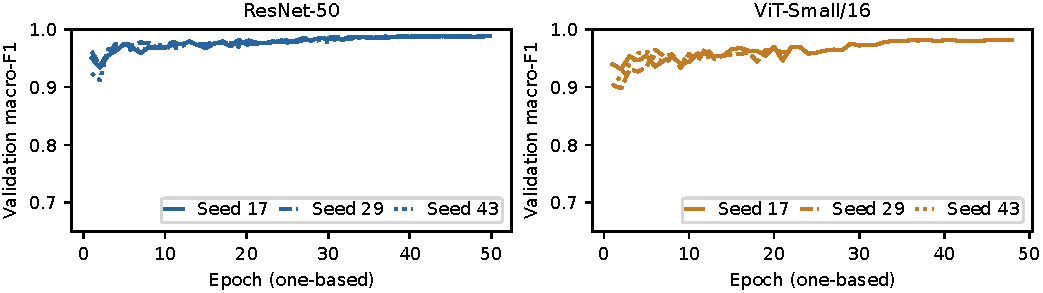
\includegraphics[width=\textwidth]{figures/learning_curves_compact.pdf}
\caption{Validation macro-F1 from the original training event logs. Line styles distinguish the three seeds within each model. Epochs are one-based, and the vertical scale spans 0.65--1.00. All points are validation measurements.}\label{fig:learning}
\end{figure}
\subsection{Optimization and recorded environments}
AdamW updates all trainable parameters with weight decay 0.05 and no label smoothing. A batch of 32 and two gradient-accumulation steps give an effective global batch of 64. Two warm-up epochs precede cosine decay, with a minimum learning-rate ratio of 0.01 and a maximum of 50 epochs. Early stopping uses validation macro-F1, patience ten, and minimum improvement 0.0001. Horizontal and vertical flips each have probability 0.5 and are deterministically keyed by source, epoch, and seed. Table~\ref{tab:models} gives the model-specific learning rates and representations.

The recorded ResNet environment uses Python 3.12.14, PyTorch 2.13.0, torchvision 0.28.0 and CUDA 13.0. The ViT environment uses Python 3.12.3, PyTorch 2.6.0+cu124, torchvision 0.21.0+cu124 and CUDA 12.4. Both record NumPy 1.26.4, SciPy 1.17.1, scikit-learn 1.9.0, Pillow 12.3.0, PyYAML 6.0.3 and Weights \& Biases 0.29.0. These versions describe the environments in the experiment artifacts; the manuscript-build runtime is documented separately. GPU precision resolved to bfloat16.

\section{Full Condition Summaries}
The following table reports mean $\pm$ sample SD across three training seeds. Each condition has 4,050 source images per seed. Raw cosine measures feature similarity within a model. ECDF instability places the corresponding dissimilarity in the validation different-class-control distribution. Bold marks the better model within each family-severity pair: higher accuracy, consistency, and raw cosine, or lower ECDF instability. Displayed ties are bold for both models. A value rounded to zero does not establish semantic invariance. The original condition and class CSVs in \path{supplementary/} retain full-precision per-seed values.
\begin{center}\resizebox{\textwidth}{!}{\input{tables/full_conditions.tex}}\end{center}
\subsection{Sham and control interpretation}
All three family shams have label consistency one in the stored summaries. Tiny representation differences from floating-point identity processing do not indicate an intervention effect. Different-class controls come from the source's evaluation partition and define the dissimilarity reference. Amplitude-mixing donors come from training and share the source's dataset label. Neither sham rows nor different-class controls enter the RQ3 positive class; shams are excluded from that task entirely.

The archived class-condition table retains the ten dataset classes, whose sample counts differ (Appendix~\ref{app:counts}). The separate macro-cluster confusion table groups classes for exploratory visualization. Those groups leave the training labels unchanged and have not been independently validated as a semantic taxonomy.

\subsection{Auxiliary artifacts and selection boundaries}
The archived cross-model CKA table uses one clean representation per source, paired by training-seed identifier. CKA compares sets of representations and does not establish semantic equivalence of individual image pairs. The supplementary directory retains the full original PNG and CSV collection. The following sections document gallery selection and attention rollout.

\section{High-Confidence Failures under Mild RGB Gains}\label{app:qualitative}
The gallery shows four correct-to-incorrect transitions under mild RGB gains. Each clean prediction agrees with the dataset label and has confidence at least 0.99. After transformation, the prediction switches between PermanentCrop and HerbaceousVegetation. Figures~\ref{fig:gallery1} and~\ref{fig:gallery2} retain the original sources and their recorded order.

Selection followed a deterministic rule. Eligible rows met the frozen condition policy, used mild RGB-gain or amplitude-mixing severity, had clean confidence at least 0.99, and exhibited a correct-to-incorrect transition. Rows were sorted by decreasing clean confidence, then by model, source and pair identifiers. The first four unique sources were retained. All four selected rows were RGB-gain failures. Replaying selection across all six runs reproduced the archived metadata. Since the examples were chosen for specific failure properties, they cannot estimate prevalence or represent every transformation family.

Original RGB files and transformed float32 caches were recovered from the migration backup. Their SHA-256 values match the dataset manifest and evaluation rows. The panels preserve the native 64-by-64 pixels. Confidence values are rounded to six decimal places; values close to one should not be read as certainty. The transformed images have not been independently re-annotated.
\begin{figure}[H]
\centering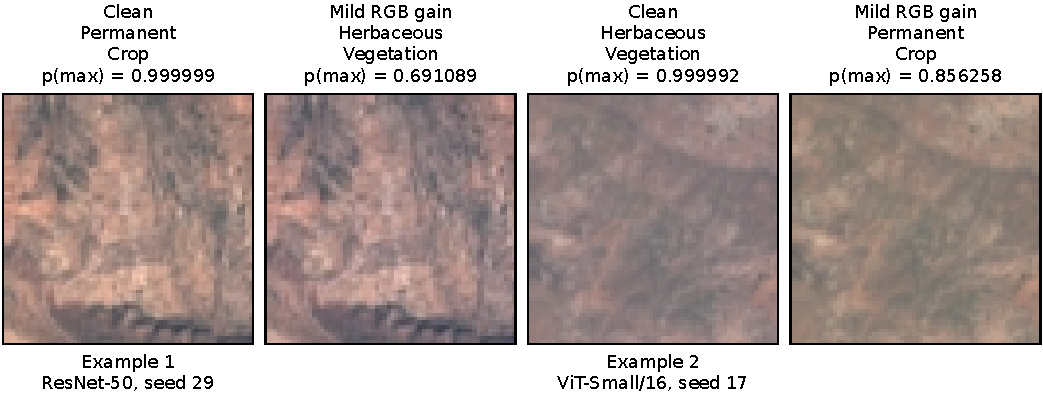
\includegraphics[width=\textwidth]{figures/qualitative_failure_gallery_1_compact.pdf}
\caption{Selected failures, examples 1 and 2, shown as two adjacent clean/transformed pairs. ResNet-50 seed29 changes from PermanentCrop to HerbaceousVegetation; ViT-Small/16 seed17 changes in the opposite direction. Each pair shows the clean input first and its recorded mild RGB-gain input second. Titles give predicted classes and maximum-softmax confidence. Clean predictions equal the dataset labels; run identifiers appear below the clean panels.}\label{fig:gallery1}
\end{figure}
Figure~\ref{fig:gallery2} continues the same deterministic selection with examples 3 and 4.
\begin{figure}[H]
\centering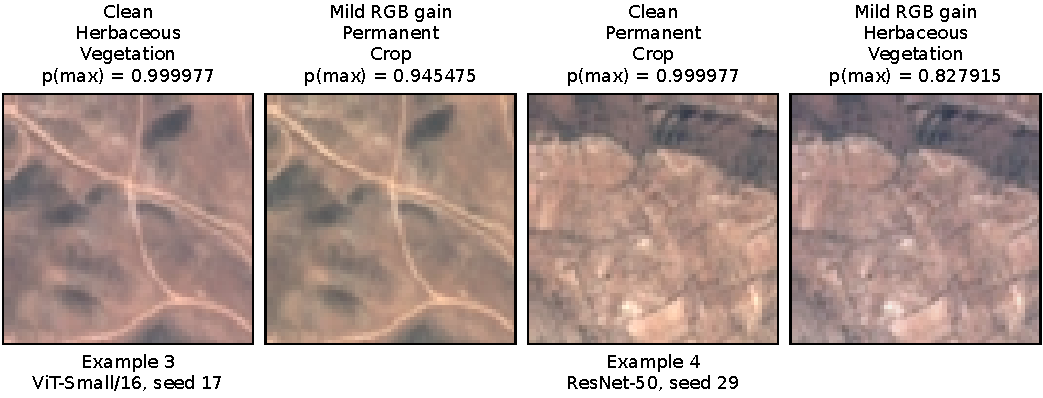
\includegraphics[width=\textwidth]{figures/qualitative_failure_gallery_2_compact.pdf}
\caption{Selected failures, examples 3 and 4, continuing the deterministic ordering in Figure~\ref{fig:gallery1} with two different sources. ViT-Small/16 seed17 predicts PermanentCrop for the transformed HerbaceousVegetation source; ResNet-50 seed29 predicts HerbaceousVegetation for the transformed PermanentCrop source. Correctness is measured against the original dataset labels.}\label{fig:gallery2}
\end{figure}
\FloatBarrier
\subsection{Interpreting the examples}
The selected pairs show class switches despite mild channel gains and high starting confidence. Their apparent visual similarity cannot establish that the original labels remain appropriate. They illustrate the benchmark's failure definition; the quantitative tables describe performance across the full evaluated populations. Example 2 is also the source selected by the archived ViT attention routine.
\section{Attention Rollout and Rendering Repair}\label{app:attention}
Attention rollout averages heads, adds identity connections, normalizes rows, and propagates attention through successive layers to approximate token information mixing~\cite{rollout}. The ViT-Small/16 seed17 example uses classification-token-to-patch rollout for gallery example 2. Each patch map is interpolated to 224-by-224 and min--max normalized separately. Rollout describes attention propagation without establishing causal pixel importance. Separate normalization also prevents interpreting color intensity as an absolute difference between clean and transformed attention.

The original plot overlays a 224-by-224 attention map on a 64-by-64 image without a shared extent. The coordinate mismatch compresses the image into one corner of the overlay. The supplementary materials preserve that PNG as a historical artifact; the figure below uses corrected coordinates.

The corrected rendering uses the same frozen ViT-Small/16 seed17 checkpoint and clean/transformed inputs. The local runtime uses \path{timm==1.0.29}, matching the recorded model-library version. One CPU forward call processed the two inputs. Both predicted classes match the archived pair, and the largest absolute difference in maximum confidence is 0.000153, below the predeclared 0.005 tolerance. The input and rollout layers share a 224-by-224 display extent. Figure~\ref{fig:attention} was visually checked at its original PNG resolution. No training, detector fitting or full-test inference was repeated.
\begin{figure}[H]
\centering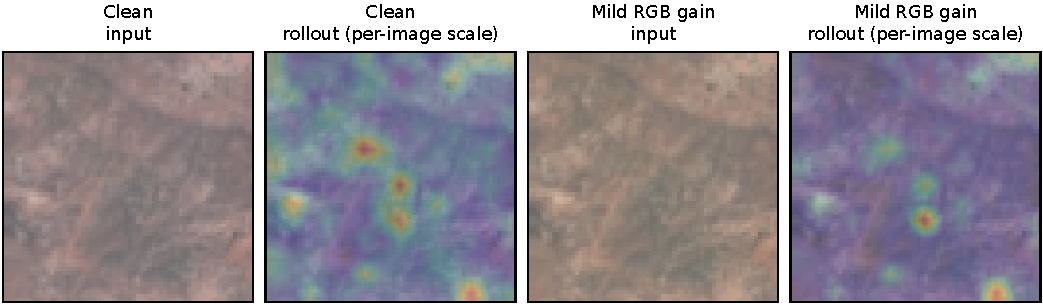
\includegraphics[width=\textwidth]{figures/attention_rollout_compact.pdf}
\caption{Corrected attention rollout for gallery example 2 using the frozen ViT-Small/16 seed17 checkpoint. The prediction changes from HerbaceousVegetation on the clean input to PermanentCrop under mild RGB gain. Panels show the clean input, clean rollout, transformed input, and transformed rollout in that order. The 64-by-64 inputs and overlays share the same coordinates. Each map is min--max normalized separately. Colors describe relative attention within each image and cannot establish an absolute change between images, causal pixel importance, or semantic label preservation.}\label{fig:attention}
\end{figure}
\section{Failure-Detector Populations and Paired Intervals}\label{app:detector}
Each eligible clean-correct source contributes nine non-sham pairs. The table below gives the resulting populations for every model and seed. Differences in failure prevalence affect the interpretation of AP even though each source receives the same nine conditions.
\begin{center}\input{tables/population.tex}\end{center}
The stored primary 95\% percentile intervals use 2,000 source-group bootstrap replicates. Both detector scores share every resampled row. The intervals are conditional on the trained checkpoint, fitted calibration detector, and fixed condition mixture, excluding uncertainty from detector refitting. They have not been adjusted for simultaneous coverage. Bold marks the largest gain for each metric within each model; interval bounds are not ranked.
\begin{center}\input{tables/delta_ci.tex}\end{center}
The gains compare the output-only baseline of transformed uncertainty and entropy with the same detector augmented by normalized representation instability. They apply to this feature comparison. Absolute per-seed scores and their uncertainty are available in \path{supplementary/detector_metrics.csv}; condition prevalence is in \path{supplementary/rq3_condition_prevalence.csv}. The primary tables report AP and AUROC separately and distinguish seed SD from the bootstrap intervals above.

\subsection{Exploratory analyses}
The archived exploratory table contains 36 defined tests across six model/seed runs, three families, and two configured metrics. Benjamini--Hochberg adjustment applies across that exploratory family, separately from the primary Holm procedure. The additional JS--ECDF Spearman correlations in \path{audit/relationships.json} were calculated after final evaluation from saved non-sham rows. Pooling severities within each run/family and repeating sources can induce association. The correlations are descriptive, without significance tests or causal interpretation.
\section{Provenance, Repairs, and Reproduction Boundaries}\label{app:provenance}
The following SHA-256 identifiers authenticate the recorded experiment. Labels and digests occupy separate lines for readability, and the machine-readable audit preserves the full strings. Repository availability and artifact authentication remain separate checks.
\begin{itemize}
\setlength{\itemsep}{1pt}
\item \textbf{Experiment protocol:}\\[-2pt] \path{cd20ca70be0619e87b2422fa99f7601c9b86578e06475f15a385903c9ed134a9}
\item \textbf{Base configuration:}\\[-2pt] \path{cc73206d4ff490bebaa9440af5689decd4a93d08038df486dadd8dfe0deb449c}
\item \textbf{Active campaign:}\\[-2pt] \path{d6dd3cabca656ef4414b165d82de1d9f45a228418a25e84e696eab9f248c7e8b}
\item \textbf{Dataset manifest:}\\[-2pt] \path{aa110365b4ad49a955680e1f8972eccd5a199946a3327f2e6a78cca0d78ced9a}
\item \textbf{Split:}\\[-2pt] \path{c678399552a928652dfa8d11aaa1288d1528fb272a0a888418e76223c29a9f0c}
\item \textbf{ResNet pretrained weights:}\\[-2pt] \path{5d061a3c593d795bfe682d9b152bafbcf550579873492def3515b46db1189888}
\item \textbf{ViT pretrained weights:}\\[-2pt] \path{c20a91d93f4757b0f581519f21ad91a875cf041764873a7a5bccc8e36f360dbf}
\end{itemize}
\subsection{Historical report-index defect}
The original \path{reporting.py} validates each representation file against its run's evaluation index. A later loop loads each run's metric and pair files but does not reassign the representation-path variable before writing the source list. Consequently, five historical entries contain the sixth run's representation digest; only the final entry is correct. The defect affects the source list. Each evaluation retains its own representation matrix, authenticated against its corresponding index.

The audit hashes each file at its explicit run path, checks evaluation and statistics digests, verifies NPZ pair ordering, and recomputes cosine and ECDF values in batches. Clean accuracy, macro-F1, condition means, failure counts, primary simple effect estimates, and AP/AUROC for all five detector scores are independently recomputed from saved outputs. Stored bootstrap intervals are authenticated against the primary statistics and their inspected implementation; a full independent rerun of the bootstrap replicates was not performed. Original files, including the incorrect historical report index, are preserved. Corrected per-run hashes are recorded in \path{audit/source_audit.json}.

The archived software-fix note documents an earlier vocabulary repair. The report validator's population wording changed from ``accepted'' to ``selected'', with the frozen protocol preserved. Python compilation passed after the repair, but pytest was unavailable on the remote runtime. The note therefore provides no evidence that the full software test suite passed there.

\subsection{Available reproduction paths}
Document reproduction needs this directory and a LaTeX engine with IEEEtran. Rebuilding assets requires the authenticated \path{all_artifacts/} tree and Python analysis packages; the qualitative panels also need the eight source/cache files recorded in the visual audit. Full experiment reproduction additionally requires the raw dataset, pretrained checkpoint binaries, resolved training configuration, software environment, pair-generation code, and appropriate compute. Regenerating transformation caches requires matching inputs and implementation. Availability and publication of these external training dependencies must be checked separately from document compilation.

Manuscript preparation did not create a Git tag, push to a remote, launch training, or repeat final-test inference. The project repository is cited in the abstract. The local baseline tag is \path{sac-campaign-v1-final}; the course's \path{v1.0-final} still needs owner confirmation. The team supplied author names, affiliation, and email addresses. All authors must approve the final submission. Administrative checks are recorded in \path{audit/qa_status.md} alongside the quantitative audit status.

\subsection{Visual revision provenance}
The scatter retains every non-sham pair, giving 109,350 observations in each model panel. The severe-condition heatmap preserves the three-seed mean of every original class/condition cell while revising grouping, labels, and color scale. Gallery selection and source/cache hashes were checked before the four original image pairs were rendered as two figures. Original report PNGs remain unchanged. Appendix~\ref{app:attention} documents the corrected attention figure and the limited replay used to create it. Figure sources, input hashes, runtime details, and logo trims are recorded in \path{audit/visual_revision.json} and \path{audit/attention_repair_status.json}.
